\documentclass{standalone}
\usepackage{tikz}
\usepackage{ctex,siunitx}
\usepackage{tkz-euclide}
\usepackage{amsmath}
\usetikzlibrary{patterns, calc}
\usetikzlibrary {decorations.pathmorphing, decorations.pathreplacing, decorations.shapes,}
\begin{document}
\small
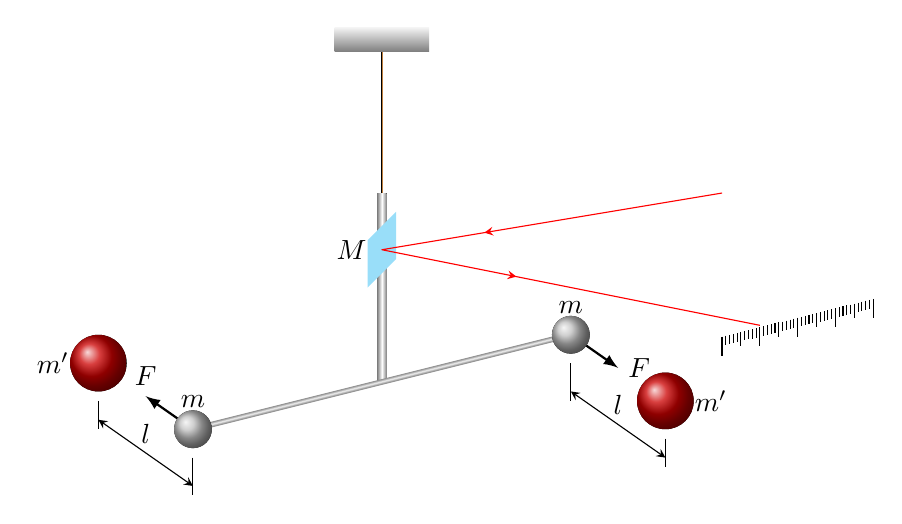
\begin{tikzpicture}[>=stealth,scale=1.2]
  \fill[left color=gray,right color=gray,middle color=white](-0.05,0)rectangle(0.05,2.0);
  \foreach \x/\y in {2/90,1.6/75,1.1/50,0.5/20}
  {
    \draw[line width=\x pt,gray!\y](-2,-0.5)--(2,0.5);
  }
  \draw[thin](-3,-0.2)--(-3,-0.5);
  \draw[thin](-2,-0.8)--(-2,-1.2);
  \draw[thin,<->](-3,-0.4)--(-2,-1.1)node[midway,above]{$l$};
  \draw[thin](3,-0.6)--(3,-0.9);
  \draw[thin](2,0.2)--(2,-0.2);
  \draw[thin,<->](3,-0.8)--(2,-0.1)node[midway,above]{$l$};
  \draw[-latex,thick](-2,-0.5)--++(-0.5,0.35)node[above]{$F$};
  \draw[-latex,thick](2,0.5)--++(0.5,-0.35)node[right]{$F$};
  \fill[ball color=lightgray](-2,-0.5)circle(0.2)node[above=1.5mm]{$m$};
  \fill[ball color=lightgray](2,0.5)circle(0.2)node[above=1.5mm]{$m$};
  \fill[ball color=red!80!black](-3,0.2)circle(0.3)node[left=2.5mm]{$m'$};
  \fill[ball color=red!80!black](3,-0.2)circle(0.3)node[right=2.5mm]{$m'$};
  \fill[cyan!40](0.15,1.8)--(-0.15,1.5)--(-0.15,1.0)--(0.15,1.3);
  \draw[double=brown,ultra thin,double distance=0.1pt](0,2.0)--(0,3.5);
  \fill[top color=lightgray!20,bottom color=gray](-0.5,3.5)rectangle(0.5,3.75);
  \draw[thin,red,line join=round,postaction={decorate},decoration={markings,mark=between positions 0.33 and 0.9 step 0.33 
  with {\arrow{>}}}](3.6,2.0)--(0,1.4)node[left=2pt,text=black]{$M$}--(4,0.6);
  \foreach \x in {-1,0,1,2}
  {
    \draw(4+0.4*\x,0.58+0.1*\x)--++(0,-0.2);
    \draw(4+0.4*\x+0.2,0.58+0.1*\x+0.05)--++(0,-0.15);
    \foreach \y in {1,2,3,4,6,7,8,9}
      { \draw(4+0.4*\x+0.04*\y,0.58+0.1*\x+0.01*\y)--++(0,-0.10); }
  }
  \draw(5.2,0.88)--++(0,-0.2);
\end{tikzpicture}
\end{document}